\documentclass{article}
\usepackage[T1]{fontenc}
\usepackage[utf8]{inputenc}

\usepackage{cmbright}
\usepackage[T1]{fontenc}

\usepackage{multicol}

\usepackage{amsmath}
\usepackage{amsfonts}
\usepackage{amssymb}
\usepackage{tikz}
\usepackage{graphicx}
\graphicspath{  {./images/} }
\setlength{\parindent}{0pt}
\usepackage{changepage}
\usepackage{verbatim}
\usepackage{physics}
\usepackage{derivative}
\usepackage{bm}
\usepackage[colorlinks=true, linkcolor=blue, urlcolor=blue, citecolor=blue, anchorcolor=blue]{hyperref}

\addtolength{\oddsidemargin}{-.25in}
\addtolength{\textwidth}{0.5in}

\makeatletter
\newcommand*\bigcdot{\mathpalette\bigcdot@{.5}}
\newcommand*\bigcdot@[2]{\mathbin{\vcenter{\hbox{\scalebox{#2}{$\m@th#1\bullet$}}}}}
\makeatother

\DeclareMathOperator{\di}{d\!}
\newcommand*\Eval[3]{\left.#1\right\rvert_{#2}^{#3}}

\newcommand{\uvec}[1]{\boldsymbol{\hat{\textbf{#1}}}}
\newcommand{\vr}[1]{\textbf{#1}}

\newcommand{\thus}[0]{\; \; \longrightarrow \; \;}

\newcommand{\lag}{\mathcal{L}}
\newcommand{\ham}{\mathcal{H}}

\title{SNR Expectation vs. Noise Values}
\author{Ryan Liu}
\date{Last updated: May 30, 2021}

\begin{document}

\maketitle

\section{Overview}

The expectation value of the SNR is calculated in the absence of noise. Because simulations of noise are Gaussian, when averaged over a large number of simulations including noise the average SNR should be approximately equal to the expectation SNR. In this document, we confirm whether this assumption is true, and if not, where discrepancies may stem from. 

\section{Results}

From Document (2.3), we know that multiple simulations of detecting the same waveform signal over random noise produces a roughly normal distribution. Therefore, the most straightforward way to determine whether the expectation value aligns with this distribution is to compare it to the median of the simulated distribution.

\begin{figure}[!htb]
    \center{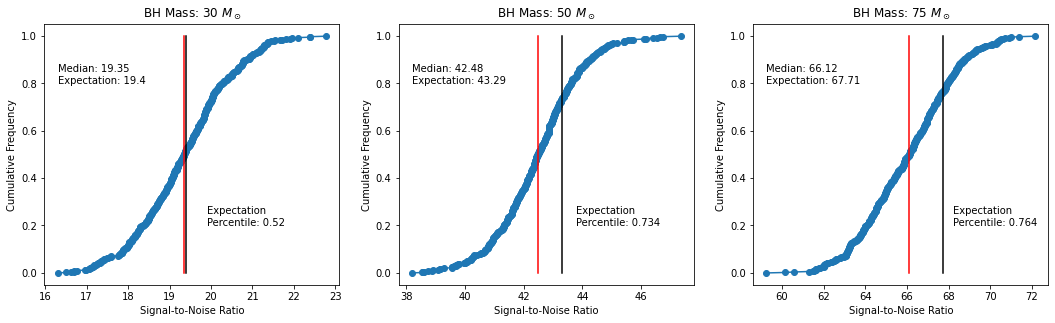
\includegraphics[width=\textwidth]{SNR15.png}}
    \caption{\label{fig:cdf} Cumulative distribution plots of 500 simulations of signal searching over Gaussian noise from the aLIGO design senstivity PSD}
\end{figure}

Interestingly, from Figure \ref{fig:cdf} we see that the expectation value is consistently higher than the median of the simulated value; furthermore, the discrepancy increases as the mass of the black hole increases. This means that adding noise over the generated signals has a net negative effect on the detection strength. \\

\begin{figure}[!htb]
    \center{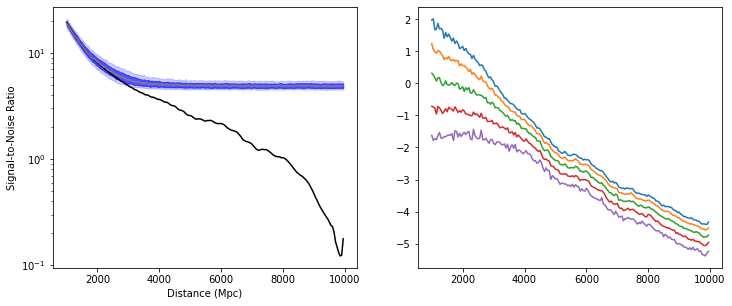
\includegraphics[width=\textwidth]{SNR16.png}}
    \caption{\label{fig:distance} (Left) SNR of a 30 $M_\odot$ BH merger at aLIGO design sensitivity; the black line denotes the expectation SNR and the blue bands give the 25\% to 75\% and 10\% to 90\% SNR values in 500 simulations with added noise. (Right) Difference between expectation value and 90th, 75th, 50th, 25th, and 10th percentiles of simulations}
\end{figure}

Repeating the simulations over many distances, it can be seen that the difference between the expectation SNR and simulated SNR drops relatively steadily. At small distances, the expectation and simulated SNRs agree closely with each other, but the spread in simulated SNRs is larger. At large distances, when the maximum SNR of Gaussian noise (as calculated in Document 2.3) is significantly higher than the expectation SNR, the added GW signal does not seem to impact the reported SNR at all; additionally, the spread in values is smaller and roughly consistent.     

\begin{figure}[!htb]
    \center{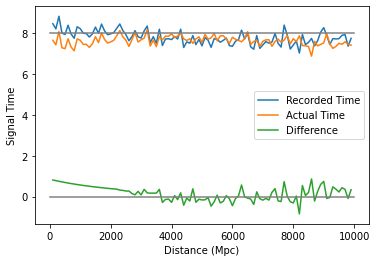
\includegraphics[width=3in]{SNR17.png}}
    \caption{\label{fig:time} Time at which the GW signal for a 30 $M_\odot$ black hole merger is inserted and detected in 16 seconds of generated noise from aLIGO design sensitivity; 100 simulations were conducted at each distance, and the mean times are plotted}
\end{figure}

When looking at discrepancies between the time stamp at which a GW signal is detected and when it was actually inserted into a simulated stretch of noise, we see in Figure \ref{fig:time} that there is a clear distinction in the pattern when signals become undetectable over noise, which occurs at approximately 3 Gpc in the figure. Before that cutoff, the difference steadily decreases with increasing distance, as expected given that the redshift effect stretches out signals; above the cutoff, the difference is random, meaning that there is no correlation between the actual location of the signal and the maximum SNR detected. \\

However, it is surprising that there is a consistent positive difference between the time of detection and time of insertion for detectable GW signals. The maximum SNR should be achieved when the template waveform and the signal directly overlap with each other, as any other arrangement will lead to destructive interference. There does not appear to be any obvious explanation for this. 

\end{document}